\documentclass[12pt,a4paper]{article}
\usepackage{pgf}
% \usepackage[condensed,math]{kurier}
% \usepackage[T1]{fontenc}
\usepackage{svg}
\usepackage{tikz}
\usepackage{stanli}
\usepackage{afterpage}
\usepackage{multirow}
\usepackage{subfig}
\usepackage{pgfpages}
\usepackage{listings}
\usepackage{rotating}

\usepackage{xcolor}

\definecolor{codegreen}{rgb}{0,0.6,0}
\definecolor{codegray}{rgb}{0.5,0.5,0.5}
\definecolor{codepurple}{rgb}{0.58,0,0.82}
\definecolor{backcolour}{rgb}{0.95,0.95,0.92}

\lstdefinestyle{mystyle}{
    backgroundcolor=\color{backcolour},   
    commentstyle=\color{codegreen},
    keywordstyle=\color{magenta},
    numberstyle=\tiny\color{codegray},
    stringstyle=\color{codepurple},
    basicstyle=\ttfamily\footnotesize,
    breakatwhitespace=false,         
    breaklines=true,                 
    captionpos=b,                    
    keepspaces=true,                 
    numbers=left,                    
    numbersep=5pt,                  
    showspaces=false,                
    showstringspaces=false,
    showtabs=false,                  
    tabsize=2
}

\lstset{style=mystyle}

%\usepackage{times}


\pgfpagesdeclarelayout{boxed}
{
	\edef\pgfpageoptionborder{0pt}
}
{
	\pgfpagesphysicalpageoptions
	{%
		logical pages=1,%
	}
	\pgfpageslogicalpageoptions{1}
	{
		border code=\pgfsetlinewidth{2pt}\pgfstroke,%
		border shrink=\pgfpageoptionborder,%
		resized width=.9\pgfphysicalwidth,%
		resized height=.9\pgfphysicalheight,%
		center=\pgfpoint{.5\pgfphysicalwidth}{.5\pgfphysicalheight}%
	}%
}

\pgfpagesuselayout{boxed}


% Language setting
% Replace `english' with e.g. `spanish' to change the document language
\usepackage[english]{babel}
\usepackage{csvsimple}
% Set page size and margins
% Replace `letterpaper' with `a4paper' for UK/EU standard size
\usepackage[a4paper,top=2cm,bottom=1.5cm,left=1.5cm,right=1.5cm]{geometry}

% Useful packages
\usepackage{amsmath}
\usepackage{graphicx}
\usepackage[colorlinks=true, allcolors=blue]{hyperref}

\title{}
\author{}
\date{}

\begin{document}

\newcommand{\subf}[2]{%
    {\small\begin{tabular}[t]{@{}c@{}}
                #1 \\#2
            \end{tabular}}%
}

\begin{titlepage}
    \begin{center}
        \vspace*{3cm}

        \Huge
        \textbf{Simulation and Models: Report}

        \vspace{0.3cm}
        \Huge
        Project 1

        \vspace{0.8cm}
        \large

        %INSTRUCTED BY: MRS. A.A.S.KAUSHLYA


        \vspace{0.5cm}
        \LARGE


        \vspace{1.5cm}

        \textbf{}
        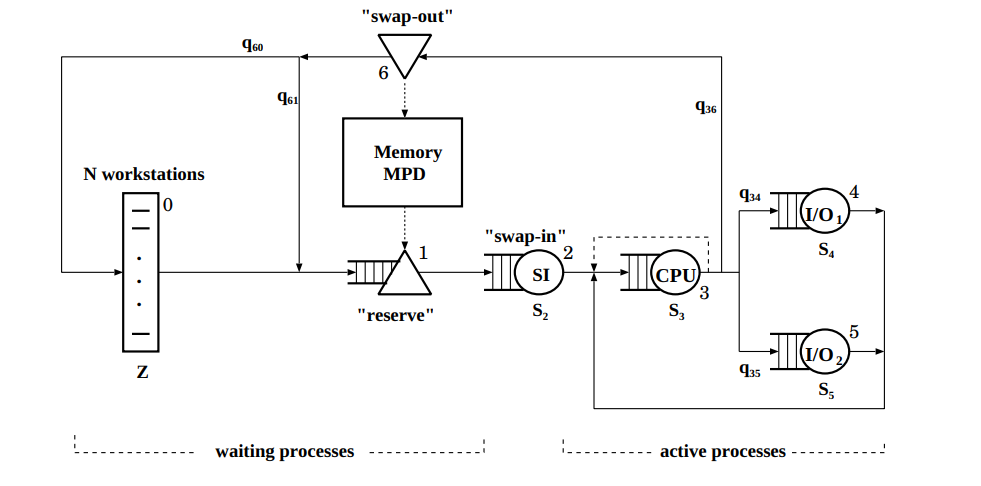
\includegraphics[width=0.8\textwidth]{./Images/model.png}

        \vfill



        \vspace{0.8cm}



        \Large




    \end{center}
    \Large
    \begin{tabbing}
        \hspace*{1em}\= \hspace*{8em} \= \kill % set the tabbings
        \> Name:\>  \textbf{Matteo Ielacqua} \\
        \> ID:\>  \textbf{839241} \\
    \end{tabbing}

\end{titlepage}



\section{Description of the simulator}
In this section a brief analysis of the code and other technical aspect of the simulator will be discussed.
\subsection{A Brief description}
The simulator generate and handle 2 type of events: an arrival of a client at a specific station or its departure.
\subsubsection{Delay station}
The delay station is an infinite server in which all the clients are served at the same time with a service time of 5000ms. When a client arrives at this station it is immediately scheduled for leaving, with a time that is has a negative exponential distribution with mean 5000ms. When a client leave it is scheduled for arrival to the reserve station.
\\
\subsubsection{Reserve station}
The reserve station is a FCFS station with instantaneous service time and a cap on how many clients can enter the system. So when the system has fewer clients than the maximum allowed by the MPD parameter it schedules an immediate departure whenever a client arrives, vice versa it will hold the client inside until the swap out complete a departure. When a client leaves it is scheduled for arrival to the swap in station.

\subsubsection{Swap in}
The swap in station is managed with an FCFS policy with a service time that is a random variable whose distribution is a negative exponential with a mean of 210 ms. When a client arrive and the station is free it is immediately scheduled for leaving using the service time distribution, instead if the station is occupied it is queued for later processing when all the other clients in the queue are served. When a clients leave it is scheduled for arrival at the CPU

\subsubsection{CPU}

The cpu is a round robin policy station with a service time that is a random variable distributed as a hyper exponential, the service times associated to this distribution are $u_1=15ms$ and $u_2=75ms$ with the corresponding weights $\alpha_1=0.8$ and $\alpha_2=0.2$. When a client arrives if it finds the station empty it's immediately processed, otherwise it's enqueued for later processing. The client stand in process for a time equal to $\min\{R,\delta\}$ where R is the remaining service time (given to the client the first time it entered in process using the hyper exponential distribution) and the parameter $\delta$ that is a "time slice" of 2.7 ms, when the remaining service time is 0 the client leaves the station, this behavior implement the round robin policy. When the departure occurs the client can be sent in one of the IOs or at the swap out. 

\subsubsection{IO}

Both IO1 and IO2 are FCFS stations (as the swap in), whose service times are random variables with negative exponential distribution with means $E[S_{IO_1}] = 180ms$ and $E[S_{IO_2}]= 40ms$. When a client leaves the stations it is scheduled for arrival at the CPU.

\subsubsection{Swap Out}
The swap out is a FCFS station with service time 0, so whenever client arrives it is immediately scheduled for departure. When a client leaves, the counter of the processes in the system (held from the swap in) is decremented, and then it can go to the delay station or to the swap in.

\subsection{Events}
The simulator is designed to manage a range of events within this system, with a particular focus on two crucial types: the arrival of a client and the departure. Each event type has a distinct impact on the simulator's state, influenced by the specific target under consideration.
\subsubsection{Delay station}

\textbf{Departure from the delay station}: The client leaving the delay station will be scheduled for arrival to the Reserve station.
\\
\textbf{Arrival at the delay station}:
an arrival will trigger a departure with a certain delay, that is a Random Variable with a negative exponential distribution with expected value of 5000 ms
\\
\subsubsection{Reserve station}
\textbf{Arrival at the Reserve station:} if the counter of the process allocated in the system is less than the MPD. Then the  arrival event is immediately scheduled for the swap in. Otherwise, the information are stored in a queue and used when a process will exit from the swap out (and the counter decremented).

\subsubsection{Swap in}
\textbf{Arrival at the swap in station:} when a client arrive 2 behavior can happen: 1) the client arrives and found the queue empty, then it will be immediately scheduled for departure with a delay based on an exponential RV with expected value of 210 ms. 2) the client find the station busy, then it will be enqueued for later processing with FCFS policy.
\\
\textbf{Departure from the swap in station:} a departure from the swap in will trigger an immediate arrival at the CPU.


\subsubsection{CPU}
\textbf{Arrival at the CPU}: when a process arrives at the CPU a service time based on a hyper exponential distribution is assigned and then 2 things can happen. 1) The CPU is not busy, then the current process will occupy the CPU and a departure will be scheduled for a time equivalent to the actual clock plus time slice, the same time will be decreased from the remaining service time of the process. 2) The CPU is busy, then the process will be enqueued in the process queue.
\\
\textbf{Departure from the CPU}: A process can leave the CPU only when its service time is 0. So when a departure is scheduled 2 case exists: 1) The process's service time is > 0, in this case the process is enqueued again in the process queue. 2) The process's service time is 0, in this case the next station will be randomly chosen (using proper probabilities) and the event will be scheduled as arrival for that station. If there is a process in the queue, after those operations, it will be dequeued and processed by the CPU using the same mechanism described for the arrivals.

\subsubsection{IO}

\textbf{Arrival to IO1/IO2:} in both cases an arrival will trigger a departure from the relative station that is an RV with negative exponential distribution.
\\
\textbf{Departure from IO1/IO2:} in both cases this will result in an immediate arrival event to the CPU.

\subsubsection{Swap Out}
\textbf{Arrival to swap out:} this event will trigger an immediate departure for the swap out
\\
\textbf{Departure from swap out:} this event will trigger an immediate arrival to the delay station with p 0.4 or an immediate arrival to the reserve station with p 0.6. In any case this event will decrement by 1 the counter of allocated process in the reserve station.



\subsection{Choice of the regeneration point}
In order to choose the regeneration point, it's possible to run some pilot simulation to see what is the system behaviour in the long run. Let's represent the state of the system by taking the number of customers actually present in each station at certain event. All the station but the CPU respect a markovnian distribution so each arrival or departure from those station is a suitable event to use as a regeneration point, let's then use the departure from the swap out, in order to catch a suitable state as a regeneration point a pilot run is performed, the state is catched when the tagged customer leaves the swap out station, as the tagged customer the first client that leaves the swap out is chosen for the duration of the run, after 1000 cycles this the output.
\begin{verbatim}
    NDelay:3, NReserve:7, NSwap:0, NCPU:0, NIO1:0, NIO2:9,NOUT:0, hits:18
    NDelay:5, NReserve:5, NSwap:0, NCPU:0, NIO1:0, NIO2:9,NOUT:0, hits:16
    NDelay:3, NReserve:7, NSwap:0, NCPU:0, NIO1:1, NIO2:8,NOUT:0, hits:16
    NDelay:2, NReserve:8, NSwap:0, NCPU:0, NIO1:0, NIO2:9,NOUT:0, hits:15
\end{verbatim}
Now in order to chose a suitable state as regeneration point it's mandatory to keep in mind that the CPU hasn't a markovnian distribution, the only states that can be used are the ones in which the number of client in the CPU are 0. Also another important aspect is the probability that the state is reached, a too frequent hit would mean a relatively small interval of observation leading to high variability of data, a too rare would mean long interval of observation and so a too long simulation. The last state in the output that is the state in which  the swap in , the cpu and the IO1 are empty, 2 clients are in being served at the delay station, 8 are at the reserve station  and 9 clients are at the IO2 , is hit 1 time every 66,6 passage of the tagged customer at the swap out, some trials revealed that this state was good enough to provide measures with precision lower that 0.05 (with a confidence of 0.9) if used as a regeneration point, and so will be chosen as regeneration point.

\subsection{Collection of measures}

The measure are collected using a particular type of accumulator, every time the regeneration point is met the following measure are collected:
\begin{enumerate}
    \item the areaN $N(t)$ accumulated by the station = $A_i$
    \item the duration of the regeneration cycle = $v_i$
\end{enumerate}

this measures are accumulated in 5 different variables as 
\begin{enumerate}
    \item $s_A=\sum_{i=1}^{p} A_i$
    \item $S_{AA} = \sum_{i=1}^{p} A_i^2$
    \item $s_v = \sum_{i=1}^{p} v_i$
    \item $s_{vv} = \sum_{i=1}^{p} v_i^2$
    \item $S_{Av} = \sum_{i=1}^{p} A_i*v_i$
\end{enumerate}

now define $\hat{r}=\frac{\bar{A}}{\bar{v}}$ and $\bar{Z}=\bar{A}-r*\bar{v}$ it's possible to calculate the confidence interval as 
$$Pr\{\hat{r}-t_{p-1,\alpha/2}* \frac{\hat{\sigma_Z}}{\bar{v}*\sqrt[]{p}}  \leq r \leq \hat{r}+t_{p-1,\alpha/2}* \frac{\hat{\sigma_Z}}{\bar{v}*\sqrt[]{p}} \} \approx (1-\alpha)$$
knowing that 
$$\frac{\hat{\sigma_Z}}{\bar{v}*\sqrt[]{p}} = \sqrt[]{\frac{p}{p-1}}*\frac{\sqrt[]{\hat{s}_{AA}-2\hat{r}\hat{s}_{av}+\hat{r}^2\hat{s}_{vv}}}{\hat{s}_v}$$

The collection of measure will be done until almost 40 samples are collected and the precision reached by the confidence interval $\frac{\Delta}{\bar{Y}} \leq \epsilon$ where $\epsilon = 0.05$, this overall process count as one simulation with one seed. 

\section{Simulation results}
The following subsection will illustrate 4 different scenarios of execution:
\begin{enumerate}
    \item Default scenario: the CPU has a Hyper exponential distribution of service time and a fixed slice time of 2.7 ms.
    \item NegExp scenario: the CPU has a negative exponential distribution of service time and a fixed time slice of 2.7 ms.
    \item LTCpu: the CPU has a hyper exponential distribution of service time and a fixed time slice of 2700 ms.
    \item NegExpLT: the CPU has a negative exponential distribution of service time and a fixed time slice of 2700 ms.
\end{enumerate}
Legend for Plots:
\begin{itemize}
    \item LB = Lower Bound of interval 
    \item HB = Higher bound of interval 
    \item R = point estimator
\end{itemize}

\subsection{Default scenario}
The default scenario leave the parameter untouched, so the Multi Programming Degree will be 10 and the number of clients in the system 20.

\includegraphics[width=0.9\textwidth]{./Images/meanActiveTime_Default.png}

\includegraphics[width=0.9\textwidth]{./Images/Default_CPU_meanclients.png}

\includegraphics[width=0.9\textwidth]{./Images/Default_CPU_meanwaits.png}

The table features the data extracted from the simulator after a run with seed 123456789.


\begin{table}[!ht]
    \centering
    \begin{tabular}{|l|l|l|l|l|l|l|l|}
    \hline
        Station & Measure & R & LB & HB & Samples & Precision & Expected \\ \hline
        CPU & meanclients & 1.3688 & 1.3378 & 1.3997 & 40 & 0.0226 & 1.4749 \\ \hline
        CPU & meanwaits & 5.9406 & 5.8458 & 6.0354 & 40 & 0.016 & 6.653 \\ \hline
        IO1 & meanclients & 1.2563 & 1.2305 & 1.282 & 40 & 0.0205 & 1.3486 \\ \hline
        IO1 & meanwaits & 88.118 & 86.8471 & 89.3889 & 40 & 0.0144 & 93.5942 \\ \hline
        IO2 & meanclients & 6.5397 & 6.4924 & 6.5871 & 40 & 0.0072 & 11.8747 \\ \hline
        IO2 & meanwaits & 1192.2379 & 1180.6697 & 1203.8062 & 40 & 0.0097 & 2142.6386 \\ \hline
        SWAP\_IN & meanclients & 0.8239 & 0.8061 & 0.8416 & 40 & 0.0215 & 0.868 \\ \hline
        SWAP\_IN & meanwaits & 377.0046 & 370.8504 & 383.1588 & 40 & 0.0163 & 391.565 \\ \hline
        ActiveTime & cycleTime & 4245.0492 & 4076.5579 & 4413.5406 & 40 & 0.0397 & 6630.2619 \\ \hline
    \end{tabular}
\end{table}

In the table it's possible to read the measure retrieved, along with point estimation (R) , the confidence interval (HB = Higher Bound and LB = lower bound), the Precision and the expected value calculated by the MVA algorithm. By a first look is immediately clear that the system performs better than expected by MVA, this is possible because MVA know nothing about the reserve station, that is holding some processes for being accepted in to the system. Thus reducing the mean clients per queue in the active part of the system and so lowering the response time that each process experience.

\pagebreak
\subsubsection{printout of the first 30 events processed}

\begin{lstlisting}
[Transfer](OS)Processing:J:11,OC:256.645482,Tp:D,Station:0
[Transfer](OS)Departure:J:11,OC:256.645482,Tp:D,Station:0
[Transfer](delay_station)Processing:J:11,OC:256.645482,Tp:D,Station:0
[Transfer](OS)Scheduling:J:11,OC:256.645482,Tp:A,Station:1
[Transfer](delay_station)Departure:J:11,OC:256.645482,Tp:A,Station:1
[Transfer](OS)Processing:J:11,OC:256.645482,Tp:A,Station:1
[Transfer](OS)Arrival:J:11,OC:256.645482,Tp:A,Station:1
[Transfer](RESERVE_STATION)Processing:J:11,OC:256.645482,Tp:A,Station:1
[Transfer](RESERVE_STATION)Arrival:J:11,OC:256.645482,Tp:A,Station:1
[Transfer](OS)Scheduling:J:11,OC:256.645482,Tp:A,Station:2
[Transfer](OS)Processing:J:11,OC:256.645482,Tp:A,Station:2
[Transfer](OS)Arrival:J:11,OC:256.645482,Tp:A,Station:2
[Transfer](SWAP_IN)Processing:J:11,OC:256.645482,Tp:A,Station:2
[Transfer](SWAP_IN)Arrival:J:11,OC:256.645482,Tp:A,Station:2
[Transfer](OS)Scheduling:J:11,OC:527.927291,Tp:D,Station:2
[Transfer](OS)Processing:J:3,OC:262.599360,Tp:D,Station:0
[Transfer](OS)Departure:J:3,OC:262.599360,Tp:D,Station:0
[Transfer](delay_station)Processing:J:3,OC:262.599360,Tp:D,Station:0
[Transfer](OS)Scheduling:J:3,OC:262.599360,Tp:A,Station:1
[Transfer](delay_station)Departure:J:3,OC:262.599360,Tp:A,Station:1
[Transfer](OS)Processing:J:3,OC:262.599360,Tp:A,Station:1
[Transfer](OS)Arrival:J:3,OC:262.599360,Tp:A,Station:1
[Transfer](RESERVE_STATION)Processing:J:3,OC:262.599360,Tp:A,Station:1
[Transfer](RESERVE_STATION)Arrival:J:3,OC:262.599360,Tp:A,Station:1
[Transfer](OS)Scheduling:J:3,OC:262.599360,Tp:A,Station:2
[Transfer](OS)Processing:J:3,OC:262.599360,Tp:A,Station:2
[Transfer](OS)Arrival:J:3,OC:262.599360,Tp:A,Station:2
[Transfer](SWAP_IN)Processing:J:3,OC:262.599360,Tp:A,Station:2
[Transfer](SWAP_IN)Arrival:J:3,OC:262.599360,Tp:A,Station:2
[Transfer](OS)Processing:J:2,OC:402.334526,Tp:D,Station:0
[Transfer](OS)Departure:J:2,OC:402.334526,Tp:D,Station:0
[Transfer](delay_station)Processing:J:2,OC:402.334526,Tp:D,Station:0
[Transfer](OS)Scheduling:J:2,OC:402.334526,Tp:A,Station:1
[Transfer](delay_station)Departure:J:2,OC:402.334526,Tp:A,Station:1
[Transfer](OS)Processing:J:2,OC:402.334526,Tp:A,Station:1
[Transfer](OS)Arrival:J:2,OC:402.334526,Tp:A,Station:1
[Transfer](RESERVE_STATION)Processing:J:2,OC:402.334526,Tp:A,Station:1
[Transfer](RESERVE_STATION)Arrival:J:2,OC:402.334526,Tp:A,Station:1
[Transfer](OS)Scheduling:J:2,OC:402.334526,Tp:A,Station:2
[Transfer](OS)Processing:J:2,OC:402.334526,Tp:A,Station:2
[Transfer](OS)Arrival:J:2,OC:402.334526,Tp:A,Station:2
[Transfer](SWAP_IN)Processing:J:2,OC:402.334526,Tp:A,Station:2
[Transfer](SWAP_IN)Arrival:J:2,OC:402.334526,Tp:A,Station:2
[Transfer](OS)Processing:J:11,OC:527.927291,Tp:D,Station:2
[Transfer](OS)Departure:J:11,OC:527.927291,Tp:D,Station:2
[Transfer](SWAP_IN)Processing:J:11,OC:527.927291,Tp:D,Station:2
[Transfer](OS)Scheduling:J:3,OC:691.351901,Tp:D,Station:2
[Transfer](OS)Scheduling:J:11,OC:527.927291,Tp:A,Station:3
[Transfer](SWAP_IN)Departure:J:11,OC:527.927291,Tp:A,Station:3
[Transfer](OS)Processing:J:11,OC:527.927291,Tp:A,Station:3
[Transfer](OS)Arrival:J:11,OC:527.927291,Tp:A,Station:3
[Transfer](CPU)Processing:J:11,OC:527.927291,Tp:A,Station:3
[Transfer](CPU)Arrival:J:11,OC:527.927291,Tp:A,Station:3
[Debug](CPU)Assigned burst time 9.490965185472163
[Transfer](OS)Scheduling:J:11,OC:530.627291,Tp:D,Station:3
[Transfer](OS)Processing:J:11,OC:530.627291,Tp:D,Station:3
[Transfer](OS)Departure:J:11,OC:530.627291,Tp:D,Station:3
[Transfer](CPU)Processing:J:11,OC:530.627291,Tp:D,Station:3
[Transfer](OS)Scheduling:J:11,OC:533.327291,Tp:D,Station:3
[Debug](CPU)Managing J:11,OC:533.327291,Tp:D,Station:3 from ready queue, remainig SV time 4.090965185472163
[Transfer](CPU)Departure:J:11,OC:530.627291,Tp:D,Station:3
[Transfer](OS)Processing:J:11,OC:533.327291,Tp:D,Station:3
[Transfer](OS)Departure:J:11,OC:533.327291,Tp:D,Station:3
[Transfer](CPU)Processing:J:11,OC:533.327291,Tp:D,Station:3
[Transfer](OS)Scheduling:J:11,OC:536.027291,Tp:D,Station:3
[Debug](CPU)Managing J:11,OC:536.027291,Tp:D,Station:3 from ready queue, remainig SV time 1.3909651854721625
[Transfer](CPU)Departure:J:11,OC:533.327291,Tp:D,Station:3
[Transfer](OS)Processing:J:11,OC:536.027291,Tp:D,Station:3
[Transfer](OS)Departure:J:11,OC:536.027291,Tp:D,Station:3
[Transfer](CPU)Processing:J:11,OC:536.027291,Tp:D,Station:3
[Transfer](OS)Scheduling:J:11,OC:537.418256,Tp:D,Station:3
[Debug](CPU)Managing J:11,OC:537.418256,Tp:D,Station:3 from ready queue, remainig SV time 0
[Transfer](CPU)Departure:J:11,OC:536.027291,Tp:D,Station:3
[Transfer](OS)Processing:J:11,OC:537.418256,Tp:D,Station:3
[Transfer](OS)Departure:J:11,OC:537.418256,Tp:D,Station:3
[Transfer](CPU)Processing:J:11,OC:537.418256,Tp:D,Station:3
[Transfer](OS)Scheduling:J:11,OC:537.418256,Tp:A,Station:5
[Transfer](CPU)Departure:J:11,OC:537.418256,Tp:A,Station:5
[Transfer](OS)Processing:J:11,OC:537.418256,Tp:A,Station:5
[Transfer](OS)Arrival:J:11,OC:537.418256,Tp:A,Station:5
[Transfer](IO2)Processing:J:11,OC:537.418256,Tp:A,Station:5
[Transfer](IO2)Arrival:J:11,OC:537.418256,Tp:A,Station:5
[Transfer](OS)Scheduling:J:11,OC:723.327231,Tp:D,Station:5
[Transfer](OS)Processing:J:6,OC:586.062860,Tp:D,Station:0
[Transfer](OS)Departure:J:6,OC:586.062860,Tp:D,Station:0
[Transfer](delay_station)Processing:J:6,OC:586.062860,Tp:D,Station:0
[Transfer](OS)Scheduling:J:6,OC:586.062860,Tp:A,Station:1
[Transfer](delay_station)Departure:J:6,OC:586.062860,Tp:A,Station:1
[Transfer](OS)Processing:J:6,OC:586.062860,Tp:A,Station:1
[Transfer](OS)Arrival:J:6,OC:586.062860,Tp:A,Station:1
[Transfer](RESERVE_STATION)Processing:J:6,OC:586.062860,Tp:A,Station:1
[Transfer](RESERVE_STATION)Arrival:J:6,OC:586.062860,Tp:A,Station:1
[Transfer](OS)Scheduling:J:6,OC:586.062860,Tp:A,Station:2
[Transfer](OS)Processing:J:6,OC:586.062860,Tp:A,Station:2
[Transfer](OS)Arrival:J:6,OC:586.062860,Tp:A,Station:2
[Transfer](SWAP_IN)Processing:J:6,OC:586.062860,Tp:A,Station:2
[Transfer](SWAP_IN)Arrival:J:6,OC:586.062860,Tp:A,Station:2
[Transfer](OS)Processing:J:3,OC:691.351901,Tp:D,Station:2
[Transfer](OS)Departure:J:3,OC:691.351901,Tp:D,Station:2
[Transfer](SWAP_IN)Processing:J:3,OC:691.351901,Tp:D,Station:2
[Transfer](OS)Scheduling:J:2,OC:939.461306,Tp:D,Station:2
[Transfer](OS)Scheduling:J:3,OC:691.351901,Tp:A,Station:3
[Transfer](SWAP_IN)Departure:J:3,OC:691.351901,Tp:A,Station:3
[Transfer](OS)Processing:J:3,OC:691.351901,Tp:A,Station:3
[Transfer](OS)Arrival:J:3,OC:691.351901,Tp:A,Station:3
[Transfer](CPU)Processing:J:3,OC:691.351901,Tp:A,Station:3
[Transfer](CPU)Arrival:J:3,OC:691.351901,Tp:A,Station:3
[Debug](CPU)Assigned burst time 9.341093139628544
[Transfer](OS)Scheduling:J:3,OC:694.051901,Tp:D,Station:3
[Transfer](OS)Processing:J:3,OC:694.051901,Tp:D,Station:3
[Transfer](OS)Departure:J:3,OC:694.051901,Tp:D,Station:3
[Transfer](CPU)Processing:J:3,OC:694.051901,Tp:D,Station:3
[Transfer](OS)Scheduling:J:3,OC:696.751901,Tp:D,Station:3
[Debug](CPU)Managing J:3,OC:696.751901,Tp:D,Station:3 from ready queue, remainig SV time 3.941093139628544
[Transfer](CPU)Departure:J:3,OC:694.051901,Tp:D,Station:3
[Transfer](OS)Processing:J:3,OC:696.751901,Tp:D,Station:3
[Transfer](OS)Departure:J:3,OC:696.751901,Tp:D,Station:3
[Transfer](CPU)Processing:J:3,OC:696.751901,Tp:D,Station:3
[Transfer](OS)Scheduling:J:3,OC:699.451901,Tp:D,Station:3
[Debug](CPU)Managing J:3,OC:699.451901,Tp:D,Station:3 from ready queue, remainig SV time 1.2410931396285436
[Transfer](CPU)Departure:J:3,OC:696.751901,Tp:D,Station:3
[Transfer](OS)Processing:J:3,OC:699.451901,Tp:D,Station:3
[Transfer](OS)Departure:J:3,OC:699.451901,Tp:D,Station:3
[Transfer](CPU)Processing:J:3,OC:699.451901,Tp:D,Station:3
[Transfer](OS)Scheduling:J:3,OC:700.692994,Tp:D,Station:3
[Debug](CPU)Managing J:3,OC:700.692994,Tp:D,Station:3 from ready queue, remainig SV time 0
[Transfer](CPU)Departure:J:3,OC:699.451901,Tp:D,Station:3
[Transfer](OS)Processing:J:3,OC:700.692994,Tp:D,Station:3
[Transfer](OS)Departure:J:3,OC:700.692994,Tp:D,Station:3
[Transfer](CPU)Processing:J:3,OC:700.692994,Tp:D,Station:3
[Transfer](OS)Scheduling:J:3,OC:700.692994,Tp:A,Station:6
[Transfer](CPU)Departure:J:3,OC:700.692994,Tp:A,Station:6
[Transfer](OS)Processing:J:3,OC:700.692994,Tp:A,Station:6
[Transfer](OS)Arrival:J:3,OC:700.692994,Tp:A,Station:6
[Transfer](SWAP_OUT)Processing:J:3,OC:700.692994,Tp:A,Station:6
[Transfer](SWAP_OUT)Arrival:J:3,OC:700.692994,Tp:A,Station:6
[Transfer](OS)Scheduling:J:3,OC:700.692994,Tp:D,Station:6
[Transfer](OS)Processing:J:3,OC:700.692994,Tp:D,Station:6
[Transfer](OS)Departure:J:3,OC:700.692994,Tp:D,Station:6
[Transfer](SWAP_OUT)Processing:J:3,OC:700.692994,Tp:D,Station:6
[Transfer](SWAP_OUT)Swapping out Process:J:3,OC:700.692994,Tp:A,Station:0 to DelayStation
[Transfer](OS)Scheduling:J:3,OC:700.692994,Tp:A,Station:0
[Transfer](SWAP_OUT)Departure:J:3,OC:700.692994,Tp:A,Station:0
[Transfer](OS)Processing:J:3,OC:700.692994,Tp:A,Station:0
[Transfer](OS)Arrival:J:3,OC:700.692994,Tp:A,Station:0
[Transfer](delay_station)Processing:J:3,OC:700.692994,Tp:A,Station:0
[Transfer](delay_station)Arrival:J:3,OC:700.692994,Tp:A,Station:0
[Transfer](OS)Scheduling:J:3,OC:15948.345652,Tp:D,Station:0
[Transfer](OS)Processing:J:11,OC:723.327231,Tp:D,Station:5
[Transfer](OS)Departure:J:11,OC:723.327231,Tp:D,Station:5
[Transfer](IO2)Processing:J:11,OC:723.327231,Tp:D,Station:5
[Transfer](OS)Scheduling:J:11,OC:723.327231,Tp:A,Station:3
[Transfer](IO2)Departure:J:11,OC:723.327231,Tp:A,Station:3
[Transfer](OS)Processing:J:11,OC:723.327231,Tp:A,Station:3
[Transfer](OS)Arrival:J:11,OC:723.327231,Tp:A,Station:3
[Transfer](CPU)Processing:J:11,OC:723.327231,Tp:A,Station:3
[Transfer](CPU)Arrival:J:11,OC:723.327231,Tp:A,Station:3
[Debug](CPU)Assigned burst time 32.77313247192449
[Transfer](OS)Scheduling:J:11,OC:726.027231,Tp:D,Station:3
\end{lstlisting}

\subsection{Negative Exponential scenario}

In this scenario the hyper exponential distribution used for generate the service times of the processes in the CPU is replaced by a negative exponential one with mean 27 ms. 

\includegraphics[width=0.9\textwidth]{./Images/meanActiveTime_NegExp.png}

\includegraphics[width=0.9\textwidth]{./Images/NexExp_CPU_meanclients.png}

\includegraphics[width=0.9\textwidth]{./Images/NexExp_CPU_meanwaits.png}

The table features the data extracted from the simulator after a run with seed 123456789.


\begin{table}[!ht]
    \centering
    \begin{tabular}{|l|l|l|l|l|l|l|l|}
    \hline
    Station & Measure & R & LB & HB & Samples & Precision & Expected \\ \hline
    CPU & meanclients & 1.3737 & 1.3553 & 1.3921 & 40 & 0.0134 & 1.4749 \\ \hline
    CPU & meanwaits & 5.9599 & 5.9091 & 6.0108 & 40 & 0.0085 & 6.653 \\ \hline
    IO1 & meanclients & 1.2618 & 1.2411 & 1.2824 & 40 & 0.0164 & 1.3486 \\ \hline
    IO1 & meanwaits & 88.4896 & 87.4961 & 89.4831 & 40 & 0.0112 & 93.5942 \\ \hline
    IO2 & meanclients & 6.5263 & 6.4703 & 6.5823 & 40 & 0.0086 & 11.8747 \\ \hline
    IO2 & meanwaits & 1189.8921 & 1177.9994 & 1201.7848 & 40 & 0.01 & 2142.6386 \\ \hline
    SWAP\_IN & meanclients & 0.8276 & 0.805 & 0.8503 & 40 & 0.0274 & 0.868 \\ \hline
    SWAP\_IN & meanwaits & 378.4739 & 371.0409 & 385.9069 & 40 & 0.0196 & 391.565 \\ \hline
    ActiveTime & cycleTime & 4092.1362 & 3932.7821 & 4251.4903 & 40 & 0.0389 & 6630.2619 \\ \hline
    \end{tabular}
\end{table}

This scene is typical of certain batch systems, for example a login server whose only job is to get credentials , verify it with a database and return a login response, each client require more or less the same time to be processed. In this case the Reserve Station and the time slice in the CPU are continuing to do their job, thus the performance obtained are pretty much the same of the previous case with an hyper exponential distribution.


\subsection{LTCpu scenario}

In this case the CPU quantum (time slice) has a very high value of 2700 ms, in practice is disabled and is not working anymore. This scene would happen for example if the linux kernel is recompiled with preemption disabled (a very bad thing to do in most of modern systems).
\\

\includegraphics[width=0.9\textwidth]{./Images/meanActiveTime_LTCpu.png}


\includegraphics[width=0.9\textwidth]{./Images/LTCpu_CPU_meanclients.png}


\includegraphics[width=0.9\textwidth]{./Images/LTCpu_CPU_meanwaits.png}

The table features the data extracted from the simulator after a run with seed 123456789.


\begin{table}[!ht]
    \centering
    \begin{tabular}{|l|l|l|l|l|l|l|l|}
    \hline
    Station & Measure & R & LB & HB & Samples & Precision & Expected \\ \hline
    CPU & meanclients & 2.3342 & 2.2962 & 2.3723 & 40 & 0.0163 & 1.4749 \\ \hline
    CPU & meanwaits & 115.8517 & 113.7034 & 118.0 & 40 & 0.0185 & 6.653 \\ \hline
    IO1 & meanclients & 1.5923 & 1.5685 & 1.6161 & 40 & 0.0149 & 1.3486 \\ \hline
    IO1 & meanwaits & 121.5879 & 120.1658 & 123.01 & 40 & 0.0117 & 93.5942 \\ \hline
    IO2 & meanclients & 5.2795 & 5.2262 & 5.3327 & 40 & 0.0101 & 11.8747 \\ \hline
    IO2 & meanwaits & 1047.7453 & 1037.9114 & 1057.5793 & 40 & 0.0094 & 2142.6386 \\ \hline
    SWAP\_IN & meanclients & 0.7873 & 0.7698 & 0.8048 & 40 & 0.0222 & 0.868 \\ \hline
    SWAP\_IN & meanwaits & 391.1256 & 384.3213 & 397.9299 & 40 & 0.0174 & 391.565 \\ \hline
    ActiveTime & cycleTime & 4549.8272 & 4377.613 & 4722.0414 & 40 & 0.0379 & 6630.2619 \\ \hline
    \end{tabular}
\end{table}

Without the time slice neither the response time of the system nor the mean clients at the other peripherals change much, just the response time increase a bit, the same is not true for the CPU, that is experiencing a drastic reduction of its performance. The main feature of the time slice is that it let the processes with a tiny service time to free the queue almost immediately, and they are the prevalent part of the processes in this situation in which the distribution is hyper exponential (because of the weights imposed by the problem 0.95 for 10 ms and 0.05 for 350 ms). Thus whenever a process with a large service time is processed by the CPU, it is occupied for all the duration of that process, then all the new processes that are enqueued will not be delivered until the one in process has terminated its service time, this means a drastic increase in the mean quantity of clients that are enqueued at the CPU.


\subsection{NegExpLT Scenario}

Also in this case, the cpu quantum is very high, so the preemption is disabled. But the service time of the CPU is a random variable with negative exponential distribution instead of an hyper exponential one.

\includegraphics[width=0.9\textwidth]{./Images/meanActiveTime_NegExpLt.png}

\includegraphics[width=0.9\textwidth]{./Images/NegExpLt_CPU_meanclients.png}

\includegraphics[width=0.9\textwidth]{./Images/NegExpLt_CPU_meanwaits.png}

The table features the data extracted from the simulator after a run with seed 123456789.

\begin{table}[!ht]
    \centering
    \begin{tabular}{|l|l|l|l|l|l|l|l|}
    \hline
    Station & Measure & R & LB & HB & Samples & Precision & Expected \\ \hline
    CPU & meanclients & 1.3709 & 1.3471 & 1.3948 & 40 & 0.0174 & 1.4749 \\ \hline
    CPU & meanwaits & 62.5487 & 61.8498 & 63.2477 & 40 & 0.0112 & 6.653 \\ \hline
    IO1 & meanclients & 1.2611 & 1.2334 & 1.2887 & 40 & 0.0219 & 1.3486 \\ \hline
    IO1 & meanwaits & 88.4654 & 87.1474 & 89.7833 & 40 & 0.0149 & 93.5942 \\ \hline
    IO2 & meanclients & 6.5345 & 6.4663 & 6.6027 & 40 & 0.0104 & 11.8747 \\ \hline
    IO2 & meanwaits & 1192.6374 & 1176.8699 & 1208.4049 & 40 & 0.0132 & 2142.6386 \\ \hline
    SWAP\_IN & meanclients & 0.8232 & 0.8014 & 0.8449 & 40 & 0.0264 & 0.868 \\ \hline
    SWAP\_IN & meanwaits & 376.9989 & 370.3191 & 383.6787 & 40 & 0.0177 & 391.565 \\ \hline
    ActiveTime & cycleTime & 4228.0506 & 4107.9863 & 4348.1148 & 40 & 0.0284 & 6630.2619 \\ \hline
    \end{tabular}
\end{table}

Thus the CPU became an FCFS policy station, but the variability of the service times is much lower, in fact there aren't process with very high service time like in the previous case, the result is that the mean clients are comparable to the negative exponential case when using the round robin queue. 



\subsection{Conclusion}



The four cases presented previously simulate the system with 2 different kind of jobs: process with service time distributed as a negative exponential and as an hyper exponential, respectively they could be divided in batch and interactive, since usually in a batch system the differences in terms of service time of the various tasks are lower than the interactive one. This kind of jobs are served by the system in 2 different situation: the time slice is working normally and is set at 2.7 ms (preemption is enabled), the time slice is very high and will never work (preemption is disabled). When the service time of clients is negative exponential, the presence of the time slice doesn't affect the CPU so much in terms of mean clients enqueue, but lower drastically the mean wait of the clients, but in the simulator there is a simplification, it is not considering the context switch cost. In modern CPU the context switch time is so tiny that it's influence is negligible, but if we suppose to work with very limited resource, for example in an embedded context where CPUs are not performant, disabling the preemption can reduce the cost of the context switching, in particular if the tasks have a small service time that differ not much from one another.\\
A very different situation happen when the clients have an hyper exponential service time, in this situation the time slice is really important for the system in order to work properly, in fact when disabled the mean waiting time and the mean clients in queue increase drastically, the system in this state would be unusable on a normal laptop/PC, since when the user press for example a character on the keyboard awaiting it to be visible on the screen, many milliseconds can elapse until this event can happen.\\
Another important aspect is the comparison against MVA, due to its intrinsics nature it cannot take in consideration the presence of the reserve station, this show an important impact that this station is having on the whole system, the reduction of the mean queue in the IO2 (in general in all the peripherals) and the response time of the system that otherwise would be much higher. Thus taking the MPD as a parameter and supposing to increase it ,after having reached the optimal point , the system will lower its throughput as long as the MPD increase, this behavior is known as thrashing.

\includegraphics[width=0.8\textwidth]{data/images/ThrashingDiagram.png}


\section{First validation step}
\subsection{Bottleneck analysis}
In order to start the analysis , let's show here the simplified model
used to conduct the validation.
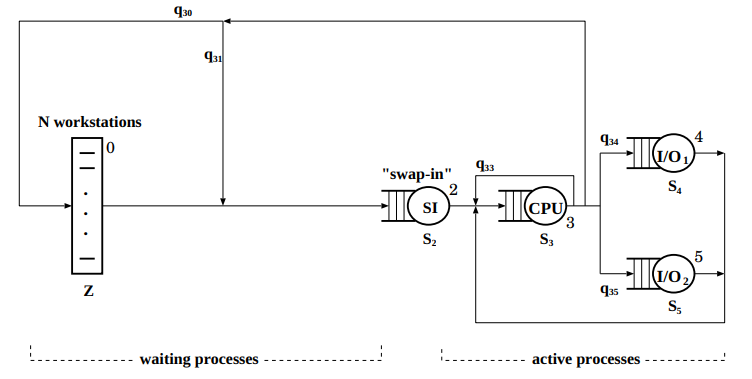
\includegraphics[width=0.8\textwidth]{Images/simplified_model.png}
\\And summarize some data:
\begin{displaymath}
    \begin{aligned}
        S_2 = 210ms  &  & S_3= 2.7ms     &  & S_4 = 40ms    &  & S_5=180ms      \\
        q_{3,0}= 0.4 &  & q_{3,1}=0.6    &  & q_{3,3} = 0.9 &  & q_{3,4}= 0.065 \\
                     &  & q_{3.5}= 0.025 &  & q_{3,6}=0.01  &  &
    \end{aligned}
\end{displaymath}
Based on this data, it becomes evident that the provided approximation is plausible. Given a process with a 0.9 probability of returning with a mean service time of 2.7, and considering our original model where clients exhibit a mean service time of 27 ms and a fixed CPU slice time of 2.7 ms, we anticipate that a customer will be rescheduled in the CPU nearly nine additional times following the initial scheduling. \\

From the previous data we can extract this matrix
\begin{displaymath}
    \begin{bmatrix}
        0     &  & 1     &  & 0   &  & 0     &  & 0     \\
        0     &  & 0     &  & 1   &  & 0     &  & 0     \\
        0.004 &  & 0.006 &  & 0.9 &  & 0.065 &  & 0.025 \\
        0     &  & 0     &  & 1   &  & 0     &  & 0     \\
        0     &  & 0     &  & 1   &  & 0     &  & 0     \\
    \end{bmatrix}
\end{displaymath}

From which we can extract the following system of equations
\begin{displaymath}
    \begin{cases}
        V_0=0.004V_3           \\
        V_2=V_0+0.006V_3       \\
        V_3=V_2+0.9V_3+V_4+V_5 \\
        V_4=0.065V_3           \\
        V_5= 0.025V_3
    \end{cases}
\end{displaymath}
with the additional equation $V_0=1$. Resolving this system lead to the computation
all $V_i$
\begin{displaymath}
    \begin{cases}
        V_0=1     \\
        V_3=250   \\
        V_2=2.5   \\
        V_4=16.25 \\
        V_5=6.25
    \end{cases}
\end{displaymath}

From this computes $V_i$ is possible to detect which of the station is the bottleneck of the system
by considering that $VbS_b= \max_i\{V_iS_i\}$, so let's compute all $V_iS_i$ and find
the greater one.

\begin{displaymath}
    \begin{aligned}
        V_2S_2= 525ms &  & V_3S_3=675ms &  & V_4S_4=650ms &  & V_5S_5= 1125ms
    \end{aligned}
\end{displaymath}
from this calculation we can say that $V_bS_b=V_5S_5=1125ms$ and so , station 5 (IO2) is
our bottleneck. Let's extract some additional information, as the total cycle time when $N=1$ ,i.e Y(1)
\begin{displaymath}
    D=\sum_{i=1}^{N}D_i=\sum_{i=1}^{N}V_iS_i + V_0S_0=7975ms
\end{displaymath}
Thus we can also calculate the saturation point $N^*$ of this system, after which we can expect
the total response time will increase.
\begin{displaymath}
    N^*=\frac{Y(1)}{V_bS_b}=\frac{D}{V_bS_b}=\frac{7975ms}{1125ms}=7.08
\end{displaymath}
\subsection{MVA analysis}
Starting from the previous matrix is possible to compute various measures using the MVA algorithm for Load Indipendent and Delay stations. In order to compute the visits vector is possible to resolve the matrix Q as system of linear equations $V=VQ$, in this case the solution comes by initializing the vector $V = [1,0,0,0,0]$ and then dot multiply it repeatly for the matrix Q. In python this can be done with the following script :\pagebreak
\begin{lstlisting}[language=python]
    matrix = np.array([
    [0,1,0,0,0],
    [0,0,1,0,0],
    [0.004,0.006,0.9,0.065,0.025],
    [0,0,1,0,0],
    [0,0,1,0,0]],np.dtype('d'))

    v = np.zeros(len(matrix))
    v[0] = 1
    for i in range(1000):
        v = v @ matrix
        pass
    for i in range(1,len(v)):
        v[i] = v[i]*(1/v[0])
        pass
    v[0] = 1
    \end{lstlisting}
Applying MVA to those values we obtain the subsequent values.

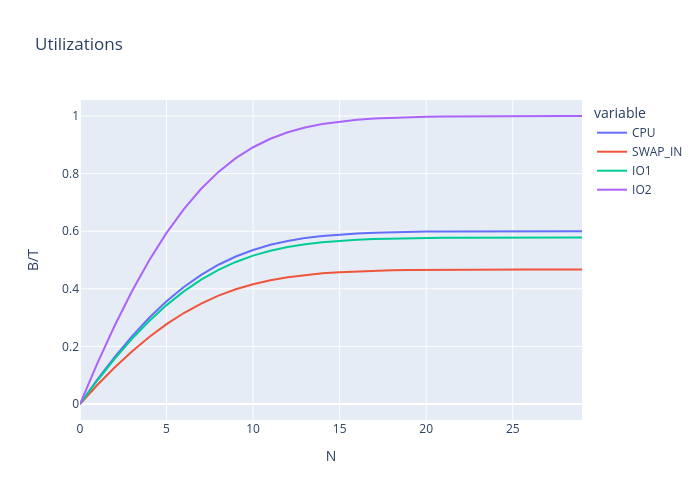
\includegraphics[width=0.9\textwidth]{./Images/Utilizations.png}\\
From the utilization functions we can conclude that the bottleneck station is IO2, as confirmed by the bottleneck analysis. Also becomes evident that after the saturation point ($N \approx7$) the growth of utilization tend to diminish despite the linear increase of N.
\\
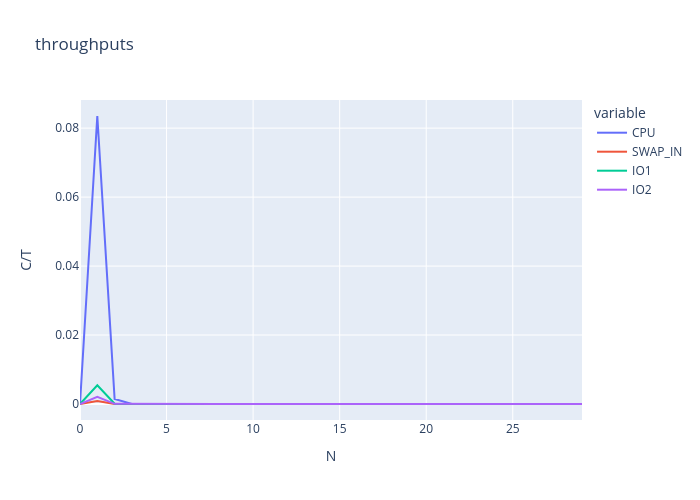
\includegraphics[width=0.9\textwidth]{Images/throughputs.png}
\\
Also from the throughputs the same statement can be reached, but with a particular observation on the CPU, that gradually stop the increasing of the throughput as N becomes larger then 7. This phenomena is similar to a very well known problem in the operative system ecosystem: thrashing. In this case the thrashing is caused by the massive use of the IO2 from the processes involved, so the throughput of the CPU will not decrease but remain steady as it will depend entirely on the process capacity of the IO2.
\\
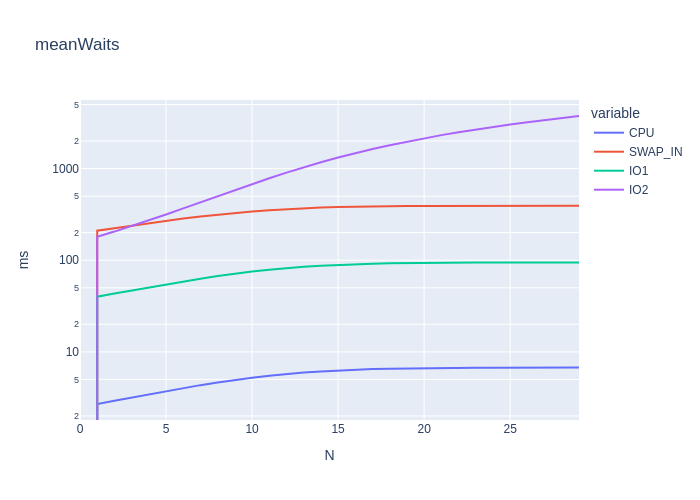
\includegraphics[width=0.9\textwidth]{Images/meanWaits.png}
\\
Mean waits also confirm that the bottleneck station is the IO2, since all other don't increase their mean wait time at the increase of N.
\\
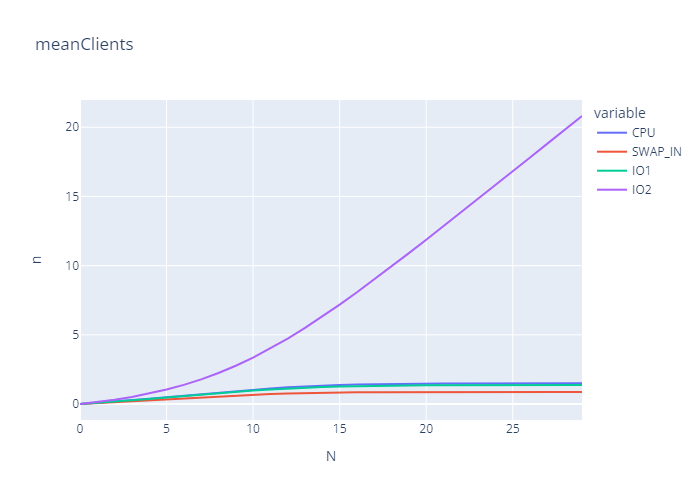
\includegraphics[width=0.9\textwidth]{Images/meanClients.png}
\\
In this graph the tendency of the IO2 station to be a bottleneck is much visible, since the customers tend to increase the queue size of the IO2 at the increase of N.

Considering the subsystem composed by IO1,IO2 and CPU we can estimate then the active time of a client with little effort, resorting to little's formula
$$
    \bar{w}= \frac{\bar{n}}{\lambda}
$$
since all the clients are coming from the swap in, then it's throughput becomes the arrival rate of the formula. The data show that with N=20 a value of 6630 should be expected.

\subsection{Comparison with the data from the simulator}
A special scenario was used to perform a comparison between the data provided by the simulator and the data provide by MVA. This scenario has special parameters. First of all burst times are distributed according to a negative exponential RV with expected value 2.7 ms, the routing probabilities contemplate the possibility of a process to return immediately to the CPU (0.9). The MPD is set to a very high value and also the time slice parameter. Since in this scenario the mean queue value is distributed differently to the other scenarios, where the MPD was limiting the number of process available in the active part of the system, a new regeneration point is adopted :every time the tagged customer leave the swap out the system must have 0 clients at the CPU, 0 at the IO1 and 16 at the IO2 and 3 at the delay station.

\includegraphics[width=0.9\textwidth]{./Images/meanActiveTime_Simplified_N20.png}



After 20 simulations, as expected, there are times in which the expected value is within the confidence interval and others not. 
\begin{verbatim}
StationCPU Measure meanwaits HitPercentage 100.0
StationCPU Measure meanclients HitPercentage 100.0
StationIO1 Measure meanwaits HitPercentage 90.0
StationIO1 Measure meanclients HitPercentage 90.0
StationIO2 Measure meanwaits HitPercentage 80.0
StationIO2 Measure meanclients HitPercentage 85.0
StationSWAP_IN Measure meanwaits HitPercentage 95.0
StationSWAP_IN Measure meanclients HitPercentage 95.0
    Activetimes HitPercentage 90.0%
\end{verbatim}

The expected value of active times, that are the focus of this simulation, were in the confidence interval 90\% of the simulations. Since the expectations are that the expected value is in the confidence interval for $N(1-\alpha)$ times or equivalently $\frac{hits}{N}*100=1-\alpha$, where hits is the number of times the expected value is in the confidence interval, the simulator can be considered a good approximation of the given model.



\section{Second validation step}
In the second validation step a different kind of effort is required, build and extract information from a Markov chain.
\subsection{States definition}
The first step is define how a state is represented. The simplest way is to consider as state a tuple of clients, each element will represent the client that are currently enqueued to each station (N\_Delay, N\_CPU, N\_IO1,N\_IO2), the swap in station is not present because it have service time 0, and so clients are processed instantaneously. 
\begin{lstlisting}[language=python]
class State:
    def __init__(self,Ndelay, Ncpu, Nio1, Nio2,cpuStage = 0) -> None:
        self.Ndelay = Ndelay
        self.Ncpu = Ncpu
        self.cpuStage = cpuStage
        self.Nio1 = Nio1
        self.Nio2 = Nio2
        self.state= [Ndelay,Ncpu,Nio1,Nio2,cpuStage]
        self.descriptor =["Ndelay","Ncpu","Nio1","Nio2","cpuStage"]
        pass
\end{lstlisting}

In this model a state is valid only if the sum of clients in each station is equal to N (the number of workstation that are present in the system). Another condition is that if there is almost 1 client in CPU, the state must be either 1 or 2.

\begin{lstlisting}[language=python,breaklines]
    def isValid(self)->bool:
        if self.Ncpu > 0:
            return (self.cpuStage == 1 or self.cpuStage == 2) and (self.Ncpu + self.Nio1 + self.Nio2 + self.Ndelay) == SystemParameters.numClients
        else:
            return (self.Ncpu + self.Nio1 + self.Nio2 + self.Ndelay) == SystemParameters.numClients
\end{lstlisting}
\pagebreak
With this simple statements is possible to define a generator of states by iterating through all the possibilities 

\begin{lstlisting}[language=python,breaklines]
def stage_enumerator(stage: int) -> list[State]:
    Ndelay = 0
    Ncpu = 1
    Nio1 = 2
    Nio2 = 3
    cpuStage = stage
    stages = [0,0,0,0]
    result = []
    while stages[Ndelay] <= SystemParameters.numClients:
        for i in reversed(range(4)):
            stages[i] += 1
            if stages[i] <= SystemParameters.numClients: break
            elif i > 0 : stages[i] = 0
            pass
        state= State(stages[Ndelay], stages[Ncpu], stages[Nio1],stages[Nio2],stage)
        if state.isValid(): result.append(state)
        pass
    return result
\end{lstlisting}

The result will be all the valid nodes for the graph, the next step is to correctly define all the possible transition in the system.

\subsection{Transition definition}
A transition is an edge in the graph, it represent the probability that the chain move from a given state to an adjacent state. A transition can be only:
\begin{itemize}
    \item A client pass from CPU to IO1 
    \item A client pass from CPU to IO2 
    \item A client pass from IO2 to CPU
    \item A client pass from IO1 to CPU
    \item A client pass from DELAY to CPU
    \item A client pass from CPU to DELAY
\end{itemize}

\begin{lstlisting}[language=python]
class Transition:   
    class TransitionType:
       UNKNOWN = -1
       CPU_TO_IO1 = 1
       CPU_TO_IO2 = 2
       IO2_TO_CPU = 4
       IO1_TO_CPU = 5
       DELAY_TO_CPU = 6
       CPU_TO_DELAY = 7
       pass

def __init__(self, head: State, tail : State) -> None:
       self.head = head
       self.tail = tail
       self.type = Transition.TransitionType.UNKNOWN
       self.detectType()
    pass
\end{lstlisting}

\pagebreak

Not all possible edges in the graph are valid, so it is necessary to impose some constraints accepted ones. Since the chain is a directed graph let's give some definitions, the head of an edge is the actual state considered, the tail is the destination of the transition. Fixed those elements a transition is valid only if:


\begin{itemize}
    \item The tail has one station with less one client than the head 
    \item The tail has one station with more one client than the head 
\end{itemize}
in this manner only the node that are one step away are considered. 

\begin{lstlisting}[language=python,breaklines]
    def transitionIsValid(self):
    #check cpu stage validity
    if self.head.cpuStage != self.tail.cpuStage:
       if self.head.Ncpu < self.tail.Ncpu and self.tail.Ncpu > 0 and self.head.Ncpu > 0: return False
       pass
    # return diff without last item that is cpu stage
    diff = np.array(self.head.state[:-1]) - np.array(self.tail.state[:-1])
    counter = 0
    # check for one step behavior
    for i in diff:
       if abs(i) > 0:
          counter+=1
       pass
    if counter > 2: return False
    return diff.max() == 1 and diff.min() == -1 and diff.sum() == 0 
\end{lstlisting}

At this point is possible to define the type of the transition simply by observing what station decremented its customer and the one that increased. A transition will be than of type: 

\begin{itemize}
    \item a transition from CPU to IO if a decrement from CPU and an increment to IO is observed and vice versa a transition from IO to CPU 
    \item a transition from CPU to Delay if a decrement from CPU is observed and an increase to Delay is observed, vice versa a transition from Delay to CPU.
\end{itemize}

\begin{lstlisting}[language=python]
    def detectType(self):
    #return so that the value remains unknown
    if not self.transitionIsValid() : return
    (decrement,increment)= self.detectMovement()
    if decrement == "ERROR" or increment == "ERROR" : return 
    elif decrement == "Ncpu" and increment == "Nio1": self.type = Transition.TransitionType.CPU_TO_IO1
    elif decrement == "Ncpu" and increment == "Nio2" : self.type = Transition.TransitionType.CPU_TO_IO2
    elif decrement == "Nio1" and increment == "Ncpu" : self.type = Transition.TransitionType.IO1_TO_CPU
    elif decrement == "Nio2" and increment == "Ncpu" : self.type = Transition.TransitionType.IO2_TO_CPU
    elif decrement == "Ndelay" and increment == "Ncpu" : self.type = Transition.TransitionType.DELAY_TO_CPU
    elif decrement == "Ncpu" and increment == "Ndelay" : self.type = Transition.TransitionType.CPU_TO_DELAY
    pass
\end{lstlisting}

So now for all transition types is possible to define a transition probability. \pagebreak

\subsubsection{Departures from CPU}

The CPU possible transition must take in consideration the current state (1 or 2) of the client in process. Starting from the departures let's define a simple, yet useful function $L_{cpu}$ (leave) that assume values 
$$L_{cpu}(H,T)=
\begin{cases}
    \frac{1}{u_1}*\alpha &  H.stage=1 \rightarrow T.stage=1 \\
    \frac{1}{u_2}*\alpha & H.stage=2 \rightarrow T.stage=1\\
    \frac{1}{u_1}*\beta & H.stage=1 \rightarrow T.stage=2 \\
    \frac{1}{u_2}*\beta & H.stage=2 \rightarrow T.stage=2\\
    \frac{1}{u_1} & H.stage=1 \rightarrow T.stage=0\\
    \frac{1}{u_2} & H.stage=2 \rightarrow T.stage=0
\end{cases}
$$
Where $u_1,u_2,\alpha,\beta$ are the constants that describe the hyper exponential of the cpu. $H$ and $T$ are the head and the tail of the transition: $H.stage=1$ means that the head is in stage 1,same for $H.stage=2$ with stage 2 and the tail that is T. Special case is $T.stage=0$ that means the tail has no client in the cpu, so alpha and beta are not considered.  

\begin{lstlisting}[language=python]
def CpuL(self):
    l = 1/SystemParameters.u1 if self.head.cpuStage == 1 else 1/SystemParameters.u2
    if self.tail.Ncpu > 0:
       l *=  SystemParameters.alpha if self.tail.cpuStage == 1 else SystemParameters.beta
       pass
    return l
\end{lstlisting}

The next steps involve to consider where the client is directed when leaving, destinations can be: Delay and IOs, also CPU to CPU are valid transitions, but useless because the values obtained from this transition will be deleted when the chain will be "normalized". So let's define function $A(H,T)$ that is arrival for a given station, $A_{IO1/2}=L_{cpu}(H,T)*q_{3,4/5}$ if the client is directed towards the IOs and $A_{delay}=L_{cpu}(H,T)*q_{3,0}$ if the client is directed to the delay station. 


\subsubsection{Arrivals to CPU}
Let's now consider all the transition that goes to the CPU i.e. arrivals. Since the service time of the swap in is 0, is possible to assume that an arrival can come from the delay station directly or from the IOs. For this purpose let $L_{delay}(H,T)$ be 
$$
L_{delay}(H,T)= H.ndelay*\frac{1}{Z}
$$

Where H.ndelay is the number of clients at the delay station and Z is the think time of the delay station and let $L_{io1}$ be
$$
    L_{io1} = \frac{1}{S_{io1}}  
$$ and let $L_{io2}$ be 
$$
    L_{io2}= \frac{1}{S_{io2}}
$$
. Let's then define a new function $A(H,T)$ for the cpu that assume values 
$$
A_{cpu}(H,T)=
\begin{cases}
    \alpha & H.stage = 0 \rightarrow T.stage = 1 \\
    \beta & H.stage = 0 \rightarrow T.stage = 2 \\
    1
\end{cases}
$$


All the transition may be described then as:

\begin{center}
    \begin{tabular}{ |c|c|c| } 
     \hline
     Station Head & Station Tail & P \\ 
     CPU & IO1 & $L_{CPU}(H,T)* q_{3,4}$ \\
     CPU & IO2 & $L_{CPU}(H,T)* q_{3,5}$\\
     CPU & Delay & $L_{CPU}*(H,T) * q_{3,0}$ \\ 
     IO1 & CPU & $L_{IO1}(H,T) * A_{CPU}(H,T)$ \\
     IO2& CPU & $L_{IO2}(H,T)* A_{CPU}(H,T)$ \\
     Delay & CPU & $L_{delay}(H,T)*A_{CPU}(H,T)$\\
     \hline
    \end{tabular}
    \end{center}

    \begin{lstlisting}[language=python]

    def DelayToCpu(self):
        l = self.head.Ndelay*(1/SystemParameters.thinkTime)
        if self.head.Ncpu == 0:
           l *= SystemParameters.alpha if self.tail.cpuStage == 1 else  SystemParameters.beta
        return l
        

    def CpuToIo(self):      
       return self.CpuL()*SystemParameters.qio1 if self.type == Transition.TransitionType.CPU_TO_IO1 else self.CpuL()*SystemParameters.qio2
        
    def CpuToDelay(self):
       return self.CpuL()*SystemParameters.qoutd
        
    def CpuToSelf(self):
    return 1/self.CpuL() *Params.qouts + 1/Params.timeSlice*self.CpuL()

        
    def IoToCpu(self):
       l = 1
       if self.head.Ncpu == 0:
          l = SystemParameters.alpha if self.tail.cpuStage == 1 else SystemParameters.beta
          pass
       return l * (1/SystemParameters.Sio1) if self.type == Transition.TransitionType.IO1_TO_CPU else l* (1/SystemParameters.Sio2)
        \end{lstlisting}


\subsection{Chain building}
The chain can be built by iterating through all nodes and edges. The easier way to do that is to apply a depth first search to the graph. The best way is to take a node as head and then iterate through all possible nodes trying to build a transition, if the transition is valid save it as edge and put the node in the frontier (if it wasn't already processed, since this graph can have cycles), at the next iteration the node will be used as head and so on. 
\begin{lstlisting}[language=python]
class ChainGenerator:
   
   def __init__(self, nodes : list[State]) -> None:
      self.nodes = nodes
      self.edges : list[Transition] = []
      self.queue = []
      self.ordered = []   
      pass

   def compute_next(self):
      ref = self.queue[0]
      self.queue.remove(ref)
      if ref in self.ordered: return
      self.ordered.append(ref)
      for node in self.nodes:
         tr = Transition(ref,node)
         if tr.type != Transition.TransitionType.UNKNOWN:
            self.edges.append(tr)
            if not node in self.ordered:
               self.queue.append(node)
               pass
            pass
         pass
      pass
\end{lstlisting}

In order to start the process, it's necessary to pick up a state from which the computation will begin, a good option is to consider in which state the system will be when the first event is processed, that is for sure the state where all the clients are at the delay station.

\subsection{Steady state solution}
In order to reach the steady state solution 3 things must be done:
\begin{enumerate}
    \item Transform the graph into a matrix 
    \item normalize the chain inside the matrix 
    \item calculate the steady state solution
\end{enumerate}

\subsubsection{Transform the graph in to a matrix}
In order to do this first step, is possible to consider the set of nodes ordered when the generation took place. Iterating through each of those nodes, is possible to build a adjacency matrix.
\begin{lstlisting}[language=python]
   def get_adj_matrix(generator: ChainGenerator):
    nodes = generator.ordered
    mat = np.zeros((len(nodes),len(nodes)))
    adj :dict = generator.chain().graph.adj
    for i in range(len(nodes)):
        ref = nodes[i]
        for j in range(len(nodes)):
            to = nodes[j]
            if to in adj[ref]:
                mat[j][i] = round(adj[ref][to]["weight"],10)
            pass
        pass
    return mat
\end{lstlisting}

\subsubsection{Normalize the chain inside the matrix}
The actual matrix is a Continuos Time Markov Chain, more precisely is an infinitesimal generator Q, but it lacks a required property $q_{ii}=\sum_{i \neq j} - q_{ij}$, so this operation is needed.

\begin{lstlisting}[language=python]
  def balance_ctmc(mat : np.ndarray[np.ndarray]) -> np.ndarray:
    copy = mat.copy()
    for i in range(len(mat)):
        copy[i][i] = -copy[i].sum()
        pass
    return copy
    pass
\end{lstlisting}

\subsubsection{Calculate the steady state solution}

In order to calculate the steady state solution, is possible to resort to this equation $\pi Q=0$  just by adding the normalization condition $\sum_i \pi_i = 1$ And transform it in a form of type $Ax=b$. First is necessary to transform the system, in order to take the system to a form of $Q \pi=b$ is possible to just transpose matrix Q and after add the normalization condition

\begin{lstlisting}[language=python]
    m = q.copy().transpose()
    norm = np.ones(len(m))
    m =np.vstack((m,norm))
    b= np.zeros(len(m))
    b[-1] = 1
\end{lstlisting}

then let's define the vector b, that is made of all 0 in order to respect the fist equation with last element 1 so that respect the normalization condition. Now let's resolve the system with least squared method (since the matrix Q now is not full rank).

\begin{lstlisting}[language=python]
    x = np.linalg.lstsq(m,b,rcond=None)[0]
\end{lstlisting}

x will then be the vector of solution pi that represent the steady state solution of the chain. In this case is a good practice to verify the optimality of the calculation by checking that the $\min(|Ax-b|_2 )< \epsilon$ where epsilon is $\approx 0$, the more this norm approach to 0 the more the solution is good.

\begin{lstlisting}[language = python]
    print(np.linalg.norm( (m@x) - b ,2).min())
\end{lstlisting}
\subsection{Extraction of data from the steady state solution}

From the steady state solution is possible to calculate some indices, for example the distribution of the mean clients in the stations. In order to extract the distribution of clients from the steady state solution is possible to consider that now each node has a probability (to be in that state) associated, then is possible to calculate $\bar{n}=\sum_{i}N * \pi_i$ where N is the number of clients that the station has in the state i.

\begin{lstlisting}[language=python]
    ordered = generator.ordered
    Ndelay = 0
    Ncpu = 0
    Nio1 = 0
    Nio2 = 0
    for state in ordered:
        p = x[ordered.index(state)]
        Ndelay += (state.Ndelay * p)
        Ncpu += (state.Ncpu * p)
        Nio1 += (state.Nio1 * p)
        Nio2 += (state.Nio2 * p)
        pass
\end{lstlisting}

Now in order to validate the model, is possible to introduce some small modification and compare it to the values calculated through the MVA algorithm. First let's calculate those values:
\begin{lstlisting}[language=python]
    matrix = np.array([
        [0,1,0,0,0],
        [0,0,1,0,0],
        [0.004,0.006,0.9,0.065,0.025],
        [0,0,1,0,0],
        [0,0,1,0,0]],np.dtype('d'))
       mva = MVA(matrix,[5000,0,2.7,40,180],[StationType.Delay,StationType.LoadIndependent,StationType.LoadIndependent,StationType.LoadIndependent,StationType.LoadIndependent],30)
       mva()
       meanClients = mvaToDataframe(mva.meanclients)
\end{lstlisting}
\pagebreak
Then is possible to set the parameters $u_1=u_2=27$, so the hyper exponential distribution of the CPU will decade to a negative exponential and the model become comparable with MVA. Running the program give this output , where in the left column are listed the measure calculated using the markov chain and at right (labeled as expected) there are the values calculated with MVA. 

\begin{verbatim}
Values calculated with 20 clients:
Ndelay 4.438583915356682 Expected 4.438722599034795
Ncpu 1.4842782312774234 Expected 1.4842718857968777
Nio1 1.3563127132526536 Expected 1.3563025143771892
Nio2 12.720825140111968 Expected 12.720703000791138
\end{verbatim}

Where expected are the values returned by MVA for the same measure. Now using instead the parameters given with a real hyper exponential the values obtained are 

\begin{verbatim}
Ndelay 4.431233117921113
Ncpu 1.8032526959726078 
Nio1 1.5225100786999133 
Nio2 12.243004107406223 
\end{verbatim}

that can be compared with the results provided by the simulator. Here the HB is the Higher bound of the estimated interval, LB the lower bound ,R the point estimator and expected is the value calculated from the markov chain.

\includegraphics[width=0.9\textwidth]{./Images/Markov_20.png}


\section{Simulator description}
\subsection{Brief description of the implementation}
The simulator is substantially a shell. The program loads at the beginning the skeleton of the simulator composed by an OS object. Such object hold the description of the model composed by a Round Robin station (class CPU), a delay station (class DelayStation) and all the other First Come First Served (class FCFSStation). The OS Object inherit from scheduler that hold the main event queue and manage all the operations inside the simulator. OS also inherit from the class Simulator, that substantially contains all the functions that are need to pilot the execution, such as dequeue an event , route it to the right station and so on. The environment of simulation is divided in 3 abstraction layers:
\begin{itemize}
    \item class SimulationEnvironment
    \item class SimulationResult
    \item class SimulationShell
\end{itemize}
\subsubsection{SimulationEnvironment}
This class hold the setup functions for the base system and each scenario. Scenarios are a short way to describe the regeneration point for that scenario and the parameter for the simulation (for example the cpu slice time). In all the four case described the regeneration point is the same, but the parameter (especially for the CPU) are different. This class also contains the SimulationResult data strucuture, which holds all the accumulators.
\subsubsection{SimulationResult}
SimulationResult class hold all the accumulator used to display the result of the simulator, it contains various function for register 2 particular measure of all the station involved: mean waits and mean clients. At the end of each regeneration cycle the measure are extracted from the OS class.
\subsubsection{SimulationShell}
this class hold all the functions need to make the program interactive, in the section Available commands various input can be used to manipulate the simulator. The principal facilities of this class let the user to create a Command structure, which pair a sequence of character to an action.
\subsection{Available commands}
\begin{itemize}
    \item help: display an help with all the commands
    \item verbosity <list|sourceName> [int] : let the user to select a verbosity for a source, the sources can be listed with list. Note that all the station have verbosity 1 in order to not display the actual processing of the events.
    \item start: manually start the simulator
    \item stop: manually stop the simulator
    \item init: initialize the system , it is needed after each call to scenario.
    \item clock: display the actual clock of the simulation.
    \item ne [int]: process a certain number of events
    \item seed: set the seed for the simulator
    \item hreset: reset completely the state of the simulator
    \item exit: quit the program
    \item regstats: display the statistics on hit and call of regeneration point , each hit correspond to an event that call the regeneration point, each call correspond to the regeneration point being satisfied.
    \item env: Display the environment variables (SystemParameters) that describe the scenario used for the simulator (MPD, slice ecc\dots)
    \item lstats: Display the actual status of the stations , B=busy time, O= observation time, A=arrivals,\\C=completions ,N: sysclients, W:meanWaits (sample mean), MAXN: max sysclients observed, AN: area of N (sysclients*interval), AS:area of S ((sysclients-1)*interval).
    \item lqueue <name>: Display the actual status of all the queues
    \item scenario <list|scenarioname>: set the scenario for the simulation. A brief description of the available scenario is available in the section Scenarios.
    \item nr <numCycles:0+|untilPrecisionReached:-1> <showMeasure:1|0>: compute the n regeneration cycle or stop when the requested precision (0.05) is reached (using -1 as argument). The second argument ask to display or not the measure after each regeneration cycle (0 false, 1 true).
    \item na <CPU|IO1|IO2|SWAP\_IN>: Execute the simulation until an arrival is detected to the station listed.
    \item nd <CPU|IO1|IO2|SWAP\_IN>: Execute the simulation until a departure is detected to the station listed.
    \item nn <seed:int> <numSimulations:int> <showMeasure:1|0> : Execute a fixed number of simulation reaching the precision requested every time, at the end of each simulation it will compare with MVA result and tell if the confidence interval has the true mean or not.
    \item ltgtstats: print the cycle time catch by the tagged customer
    \item lmeasures: print all the collected measure
    \item reset\_measures: manually reset all the accumulators

\end{itemize}

\subsection{Example of usages}
Use a scenario, compute values and print the measures, use sequential stopping rule, use seed 123456789 :\\ CpuSimulator --program "scenario [scenario] Default; seed 123456789; init ; nr -1 1; lmeasures", scenario can be Default,NegExp,LTCpu,NegExpLt and Markov
\\
\\
Use a scenario, compute 40 regeneration cycles and print the measures using seed 123456789 :\\ CpuSimulator --program "scenario [scenario]; seed 123456789; init ; nr 40 1; lmeasures"
\\
\\
\end{document}